\documentclass[12pt,a4paper]{article}
\usepackage{graphicx}
\usepackage[T1]{fontenc}
\usepackage[utf8]{inputenc}
\usepackage{linguex}
\usepackage{subcaption}
\def\refdash{}
\def\firstrefdash{}
\usepackage{wrapfig}
\usepackage{times}
%\usepackage{libertinus}

% cut pages:
% pdftk degree_achievements_2020.pdf  cat 1-2 output deg-ach-2p.pdf

% uncomment according to your operating system:
% ------------------------------------------------
% ------------------------------------------------
%\usepackage{mathptmx} %% use fitting times fonts also in formulas
%\usepackage{enumerate}
\usepackage{multirow}
\usepackage[dvipsnames,table,xcdraw]{xcolor}
\usepackage{amsmath,amsthm, amssymb, latexsym}
\usepackage{fancybox}
%\usepackage{calc}
%\usepackage{mathrsfs}
%\usepackage{multirow}
%\usepackage{multicol}
\usepackage[margin=2.5cm]{geometry} %[margin=0.5in]
%\usepackage{gb4e,qtree}
%\noautomath
\usepackage{stmaryrd}
%\usepackage{pifont}
\usepackage[normalem]{ulem}
\usepackage{hyperref}
\usepackage{microtype}

\usepackage{wrapfig}
\hyphenation{im-pli-ca-ture}
% \newcommand{\change}[2]{\textcolor{gray}{{\scriptsize\sout{#1}}\-}\textcolor{blue}{#2}}
 \newcommand{\change}[2]{\textcolor{black}{#2}}


\def\sk#1{\setbox1\hbox{#1}\rule[.5ex]{\wd1}{.4pt}\hspace*{-\wd1}{\box1}}
%\newcommand{\lizchange}[2]{\textcolor{gray}{{\sk{#1}}\-}\textcolor{purple}{#2}}
% \newcommand{\lizchange}[2]{\textcolor{purple}{#2}}
\newcommand{\lizchange}[2]{\textcolor{black}{#2}}

\newcommand{\cond}[1]{\textsc{#1}}
\newcommand{\GeurtsNouwen}{{GN}}
\newcommand{\sem}[1]{\llbracket{#1}\rrbracket}

%\linespread{0.98}
 \newcommand{\hand}{\ding{43}}
 \pagestyle{empty}
\setlength{\intextsep}{6pt plus 2pt minus 2pt}
\setlength{\textfloatsep}{8pt plus 2pt minus 2pt}
\setlength{\floatsep}{8pt plus 2pt minus 2pt}
\setlength{\abovecaptionskip}{2pt}
\setlength{\belowcaptionskip}{0pt}
\setlength{\abovedisplayskip}{6pt plus 2pt minus 3pt}
\setlength{\belowdisplayskip}{6pt plus 2pt minus 3pt}
% pdftk abstract_no-more_exp_v1.pdf cat 1-2 output abstract_no-more_exp_v2.pdf
\begin{document}

%Abstracts should be in PDF format and must be submitted via Oxford Abstracts.
%Abstracts must not exceed two A4 pages (2.5 cm margins on all sides, Times New Roman, font size no smaller than 12 pt), including references, examples, and figures.
%Examples should be incorporated into the text rather than included separately at the end.

\begin{center}{\vspace{-2ex}{\bf  Beyond Monotonicity: Czech NPI Licensing Under `majority'}}\\
%    Mojmír Dočekal (\href{mailto:docekal@phil.muni.cz}{docekal@phil.muni.cz}), Masaryk university
\end{center}
\vspace{-1ex}
\noindent \textbf{Background.} Negative Polarity Items (NPIs) are classically analyzed as markers of downward inferences (DIs; Ladusaw 1979), but experimental evidence is mixed. Szabolcsi et al. (2008) found no correlation between DIs and NPI licensing; later studies suggested one based on subjective judgments (Chemla et al. 2011; Denić et al. 2021). Barker (2018) instead argues that NPIs signal \textit{narrow scope} wrt. their licensor, not monotonicity. Dočekal and Chumchalová (2025) likewise found domain-sensitive licensing with upward-entailing (UE) inference patterns. But double licensing is not a \textit{genuinely} non-monotonic (NM) context, so it remains open whether NPIs can appear in \textit{empirically} NM environments (Alexandropoulou et al. 2020). The quantifier \textit{většina} (`most/majority') is ideal here: as a \textit{proportional} quantifier (Barwise \& Cooper 1981), it is neither upward- nor downward-entailing (DE), with denotation $\llbracket\textit{většina}\rrbracket(A)(B)=1$ iff $|A\cap B|>|A\setminus B|$. We report a two-part experiment on Czech \textit{sebemenší} (“least”) under \textit{většina}. If NPIs are licensed here while subjects reject both DE and UE inferences, this is stronger evidence against the DI–NPI link than DL and supports Barker 2018.\vspace{-0.5mm}

\noindent \textbf{Experiment.} \noindent The experiment consisted of an acceptability- and an inference judgment task. We hypothesized \textit{sebemenší} in the restrictor of a \textit{most}-QP would be judged acceptable despite \textit{většina} being seen as NM. Two questionnaire versions were created: \textit{acceptability-first} (N=24) and \textit{inference-first} (N=29). The acceptability part used 9 items in a $1\times3$ factorial design with conditions: DE \textit{all}, NM \textit{most}, and UE \textit{some}. We expected the descending order of the ratings: `all' > `most' > `some'.

\begin{minipage}{0.67\textwidth}

\exg.\small\textit{Všichni/Většina/Někteří} \small\textit{občané/-ů} \small\textit{se} \small\textit{sebemenší} \small\textit{vírou} \small\textit{v} \small\textit{Boha} \small\textit{chtěli/-a} \small\textit{nalezenému} \small\textit{dítěti} \small\textit{vystrojit} \small\textit{křest}.\label{dite}\\
\small all/majority/some \small citizens \small with \small \textit{sebe-}small \small faith \small in \small God \small wanted \small found \small child.\textsc{dat} \small arrange \small christening\\
\small ‘All/Most/Some citizens with even the least faith in God\\
wanted to have the found child christened.’

\end{minipage}
\hfill
\begin{minipage}{0.35\textwidth}

\ex.\label{inftaska}\small
\hspace{-6mm}\textit{A:} [All/Most/Some] of\\
the circles are in\\
the box on the right.\hspace{+5mm}

\ex.\label{inftaskb}\small
\hspace{-6mm}\textit{B:} ... of the [shapes\\
/green circles] are\\
in the box on the right.

\end{minipage}
\vspace{+0.5mm}

\noindent The inference task used a $2\times3$ factorial design: One factor was UE/DE entailment between the presented sentences ($circle\rightarrow shape$ or $circle\rightarrow green.circle$). The other factor was quantifier type (\textit{all/most/some}). Subjects were shown a set of 12 shapes: two types of shapes in red and green. The scenario was that each such set of shapes would be placed in two boxes with opaque walls, with a window in one box that concealed the colors (Fig \ref{tvary}). The task was to answer “yes” or “no” to whether Sentence A entailed Sentence B (see translated example in \ref{inftaska}, \ref{inftaskb}). We expected mostly “yes” ratings in DE scenarios for \textit{all}, UE for \textit{some}, and barely any “yes” ratings for \textit{most}.\vspace{-2mm}


\hspace{+1mm}
\vspace{-10pt}\begin{figure}[hbt!]
\centering
\begin{minipage}[t]{0.56\textwidth}
\centering
\begin{subfigure}{.31\textwidth}
  \centering
  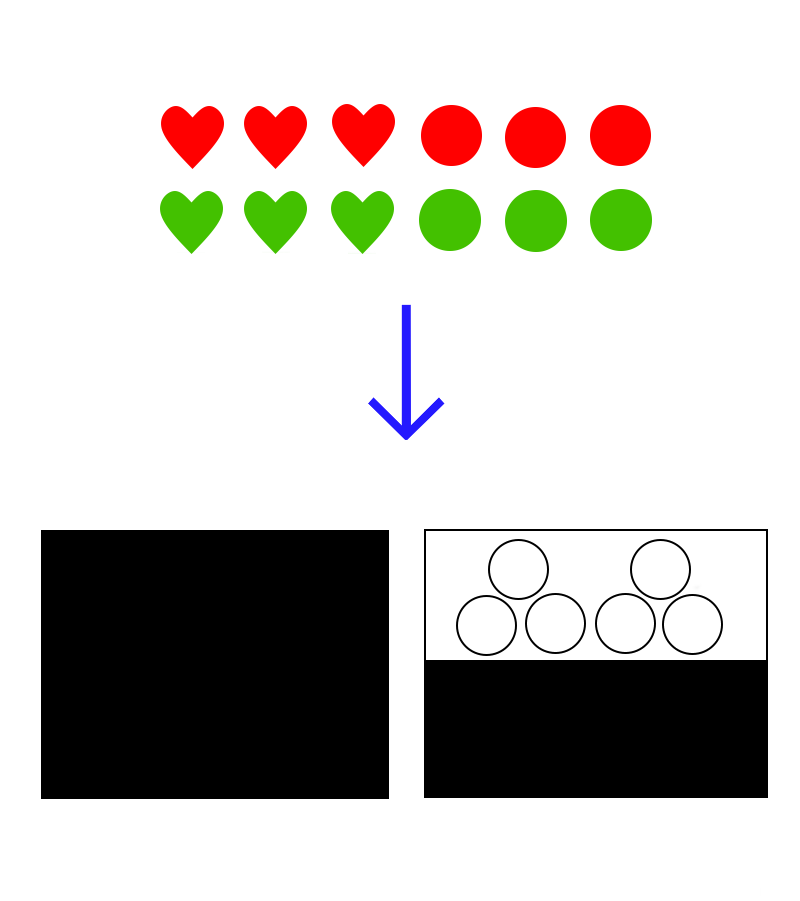
\includegraphics[width=\linewidth]{14-all.png}
  \caption{“all”}
  \label{fig:all}
\end{subfigure}
\hfill
\begin{subfigure}{.31\textwidth}
  \centering
  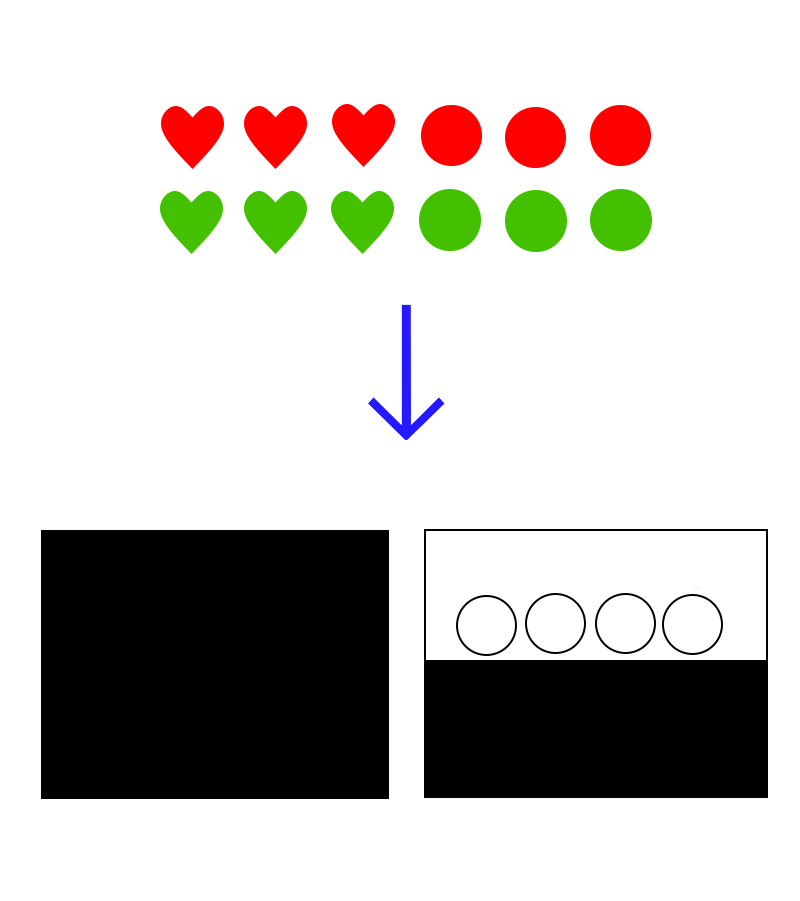
\includegraphics[width=\linewidth]{14-most.png}
  \caption{“most”}
  \label{fig:most}
\end{subfigure}
\hfill
\begin{subfigure}{.31\textwidth}
  \centering
  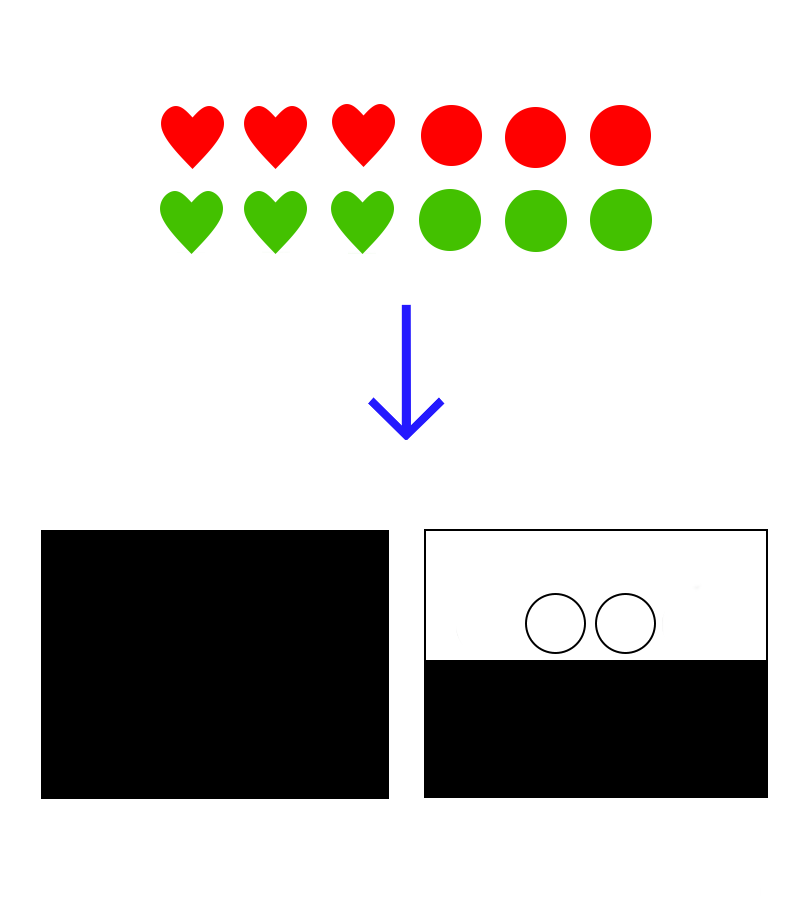
\includegraphics[width=\linewidth]{14-some.png}
  \caption{“some”}
  \label{fig:some}
\end{subfigure}
\end{minipage}
\hfill
\begin{minipage}[t]{0.40\textwidth}
\centering
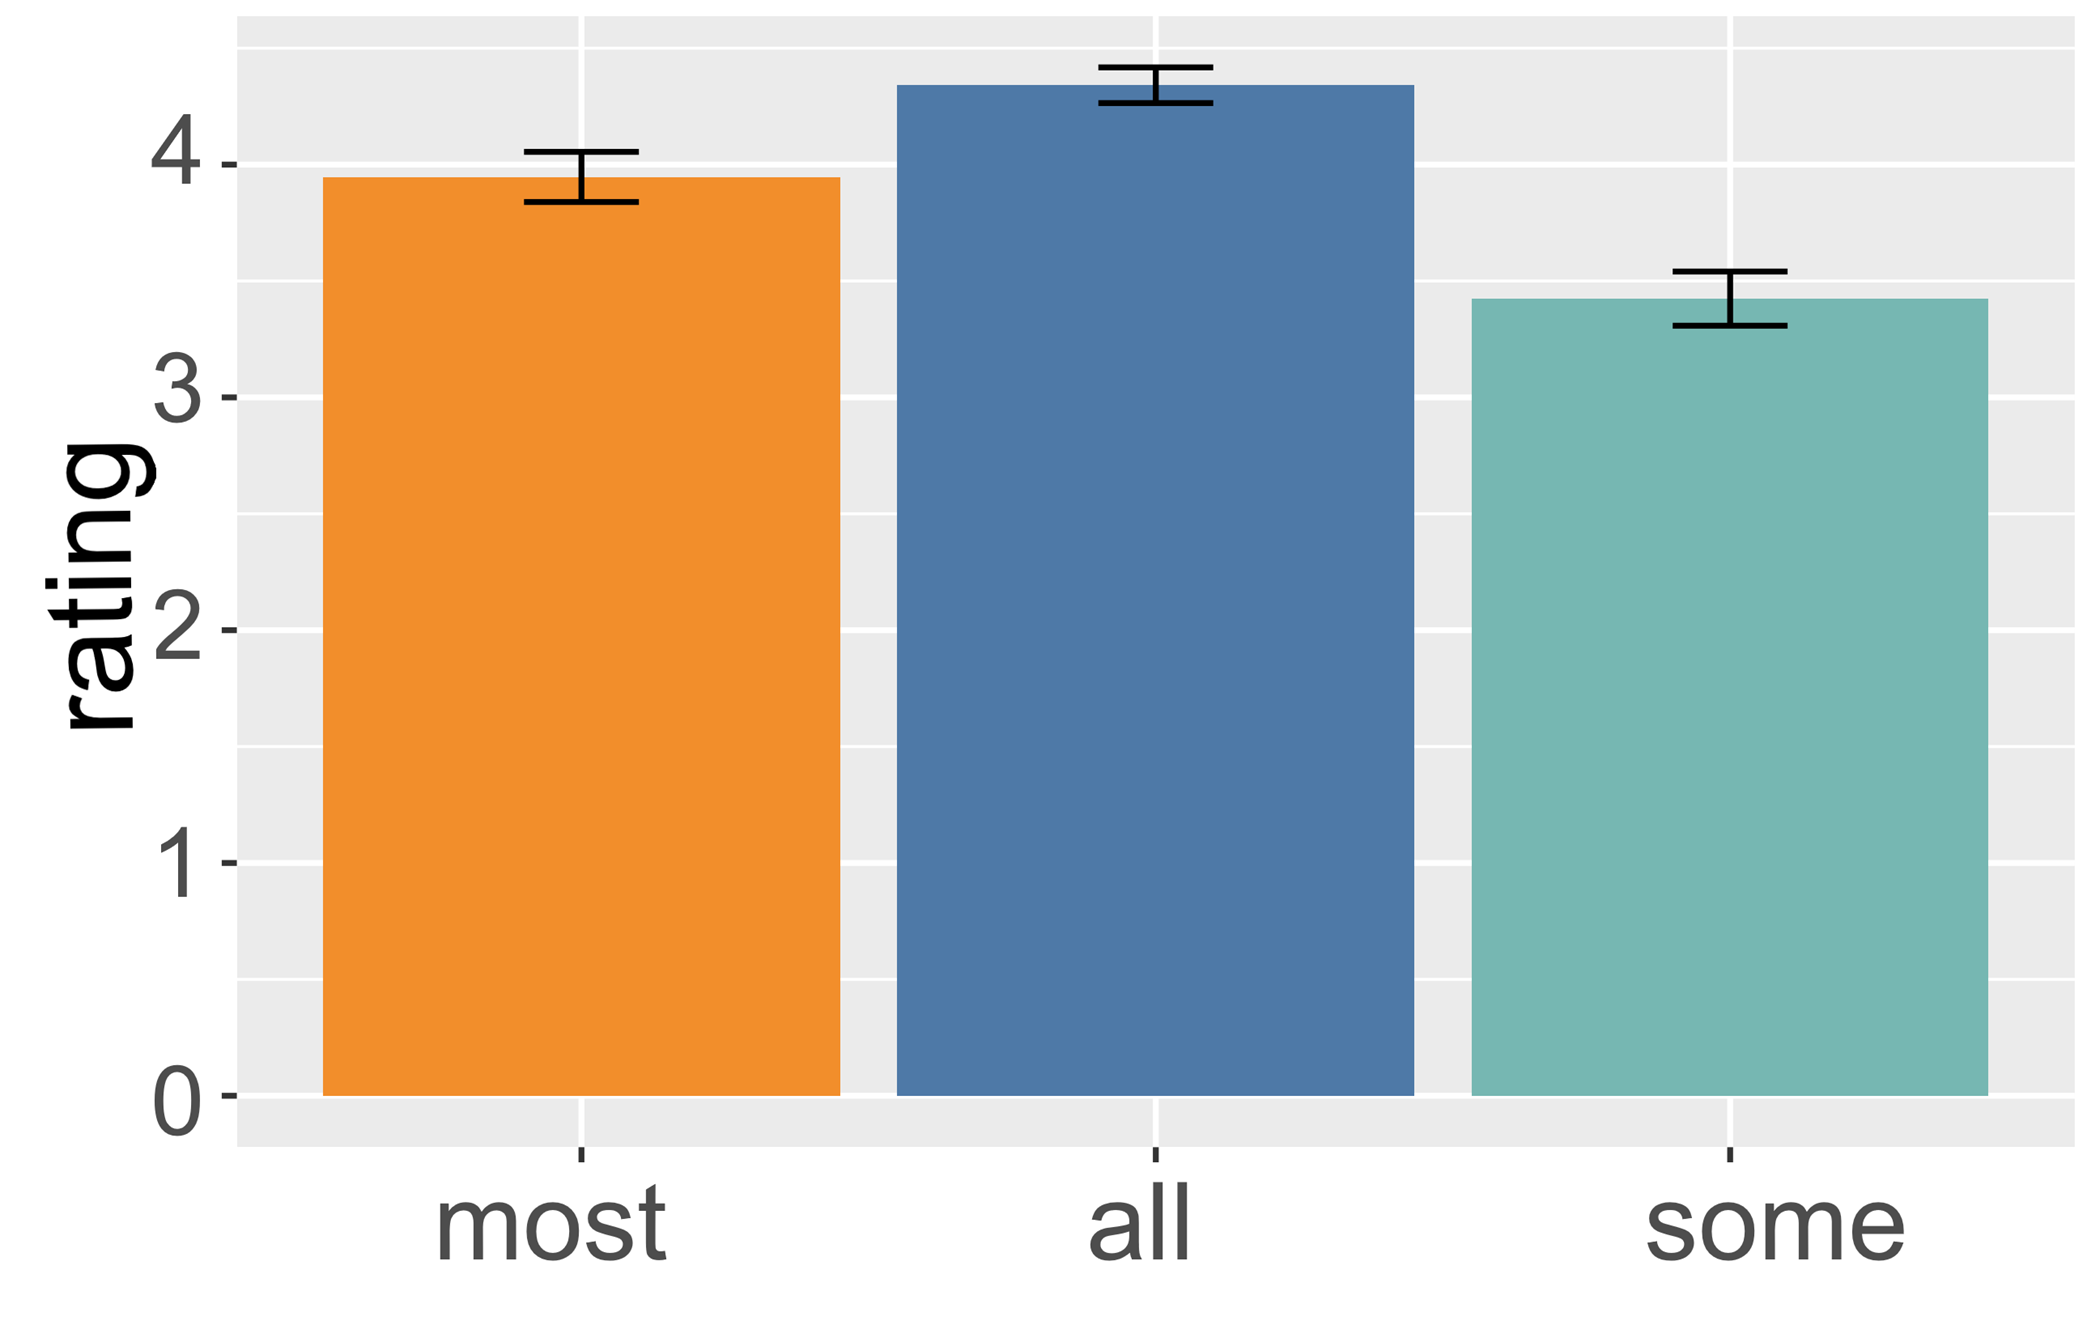
\includegraphics[width=\linewidth]{accept1.png}
\end{minipage}
\caption{Visuals for the inference task and acceptability ratings with error bars.}\label{tvary}\label{fig:acceptability}
\end{figure}

\noindent \textbf{Results.} Descriptive statistics are shown in Figures \ref{fig:acceptability} and \ref{fig:inference}. We analyzed acceptability with Bayesian linear mixed models and inference responses with Bayesian logistic mixed models (random intercepts for participants; maximal models did not converge) in \textit{R} using \textit{rstanarm} (Brilleman et al. 2018). Task order showed no credible effect ($|\hat{\beta}| < 0.3$, $\text{BF}_{01} > 4$), so we report aggregated data. In acceptability, with \textit{most} as the reference level, \textit{all} was rated credibly higher ($\hat{\beta}=0.43$, 95\% CrI [0.18, 0.67], $\text{BF}_{10}=5.14$) and \textit{some} credibly lower ($\hat{\beta}=-0.49$, 95\% CrI [-0.73, -0.24], $\text{BF}_{10}=24.6$), with extreme evidence for both effects (pd > 99.96\%). For inferences, again with \textit{most} as reference and DE as the directional baseline, participants robustly endorsed DE inferences under \textit{all} ($\hat{\beta}_{\text{UE:all}}=-8.51$, 95\% CrI $[-11.57, -5.97]$, $\text{BF}_{10}=9.20\times10^5$) and UE inferences under \textit{some} ($\hat{\beta}_{\text{UE:some}}=7.09$, 95\% CrI $[5.35, 9.09]$, $\text{BF}_{10}=3.50\times10^8$). Critically, \textit{most} showed no evidence for either inference direction (UE: $\hat{\beta}=-1.30$, 95\% CrI $[-2.85, -0.04]$, $\text{BF}_{01}=1.06$), with both DE and UE inferences rejected (DE: 6.8\%, UE: 2.3\%). Thus, \textit{most} was rated neither DE nor UE despite licensing NPIs at intermediate levels ($\mu$=3.95) between \textit{all} ($\mu$=4.34) and \textit{some} ($\mu$=3.42).

\begin{wrapfigure}{r}{0.37\textwidth}
\centering
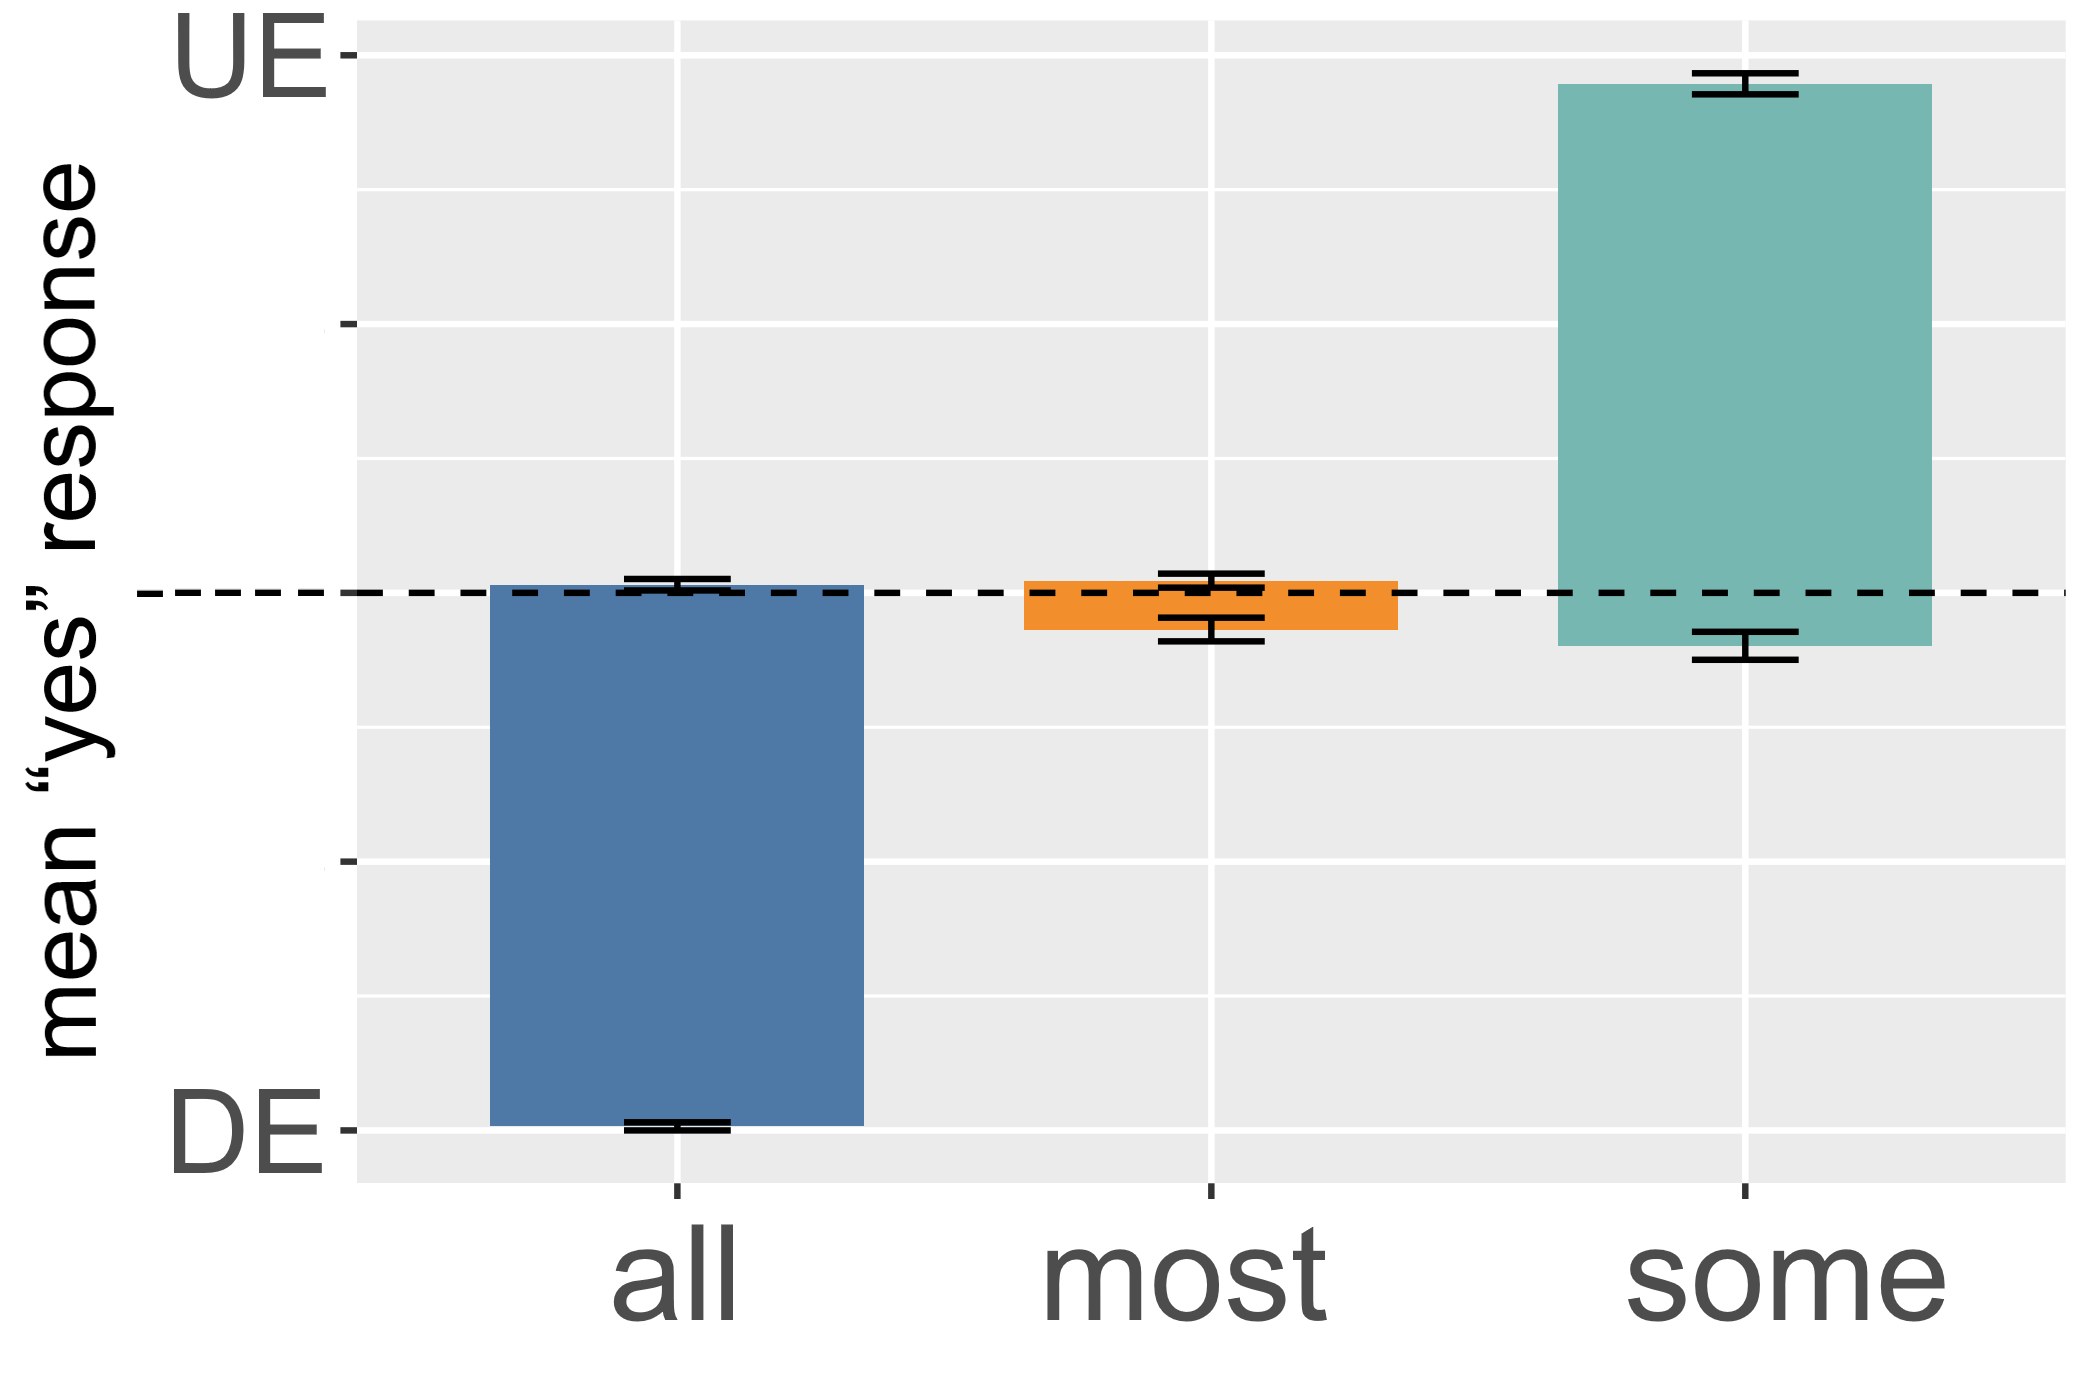
\includegraphics[width=0.39\textwidth]{infer1.png}
\caption{ \hspace{-1.8mm} \footnotesize Inference responses.}
\label{fig:inference}
\end{wrapfigure}

\noindent \textbf{Discussion.} The results reveal a critical dissociation: the NM quantifier \textit{most} licenses NPIs at intermediate acceptability levels ($\mu=3.95$) despite showing no monotonic inference pattern in the same participants (DE: 6.8\%; UE: 2.3\%). This is at odds with Ladusaw's (1979) hypothesis that DI are a synchronic licensing condition for NPIs. Unlike DL environments (Homer 2021), \textit{most} is genuinely NM in its restrictor: participants robustly rejected \textit{both} DE and UE inferences (BF$_{01}=1.06$), confirming a non-DE/non-UE environment. This dissociation provides stronger evidence against the DI--NPI link than double licensing. Participants showed \textit{extreme} evidence for DE behavior under \textit{all} (BF$_{10}=9.20\times10^{5}$) and UE behavior under \textit{some} (BF$_{10}=3.5\times10^{8}$), while \textit{most} yielded no credible preference for either direction. The acceptability gradient (\textit{all}: $\mu=4.34$ > \textit{most}: $\mu=3.95$ > \textit{some}: $\mu=3.42$) mirrors this: maximal DE licensing yields the highest acceptability, genuine NM-ity an intermediate one, and maximal UE the lowest. This pattern is incompatible with Ladusaw's synchronic DE requirement but aligns with Barker (2018): NPIs signal narrow scope wrt. their licensor (i.e., they are licensed when their wide scope does not entail their narrow scope) rather than monotonicity. Formally, from $\exists d\,[\textit{v\v{e}t\v{s}ina}_x(F(x,d)\rightarrow P(x))]$ (``there is a degree of faith such that most people satisfy $P$'') one cannot infer $\textit{v\v{e}t\v{s}ina}_x((\exists d\,F(x,d))\rightarrow P(x))$ (``most people with some degree of faith satisfy $P$'')—there may be a threshold of $d$ that guarantees $P$ (first formula true, second false). Under \textit{most}, the NPI takes narrow scope within the restrictor (\textit{sebemen\v{s}\'{i} v\'{i}rou}, `least faith'), yielding an interpretable configuration despite non-monotonicity. The results replicate Szabolcsi et al.'s (2008) null finding and extend it to a theoretically critical case: a quantifier that is \textit{empirically} NM. While NPIs may have grammaticalized in DE environments (Herburger 2023), our data show that DI is not synchronically necessary for licensing.
%\end{thebibliography}


\vspace{+1mm}
\noindent \small \textbf{References:} Alexandropoulou, S., L. Bylinina, \& R. Nouwen (2020). Is there any licensing in non-DE contexts? Proc. SuB 24(1), 35–47. $\bullet$ Barker, C. (2018). Negative polarity as scope marking. Ling. Philos. 41(5), 483–510. $\bullet$ Barwise, J. \& R. Cooper (1981). Generalized quantifiers and natural language. Ling. Philos. 4(2), 159–219. $\bullet$
Brilleman, S., M. Crowther, M. Moreno-Betancur, J. Buros Novik, \& R. Wolfe (2018). Joint longitudinal and time-to-event models via Stan. StanCon 2018. $\bullet$
Chemla, E., V. Homer, \& D. Rothschild (2011). Modularity and intuitions in formal semantics: polarity items. Ling. Philos. 34, 537–570. $\bullet$
Denić, M., V. Homer, D. Rothschild, \& E. Chemla (2021). The influence of polarity items on inferential judgments. Cognition 215, 104791. $\bullet$
Dočekal, M. \& L. Chumchalová (2025). NPIs, inferences and double licensing: experimental evidence. Talk at SuB 30, Goethe U. Frankfurt. $\bullet$
Herburger, E. (2023). On the history of NPIs and negative concord. Can. J. Linguist. 68(4), 555–589. $\bullet$ 
Homer, V. (2021). Domains of polarity items. J. Semant. 38(1), 1–48. $\bullet$ 
Ladusaw, W. A. (1979). Polarity Sensitivity as Inherent Scope Relations. PhD diss., Univ. of Texas. $\bullet$
Szabolcsi, A., L. Bott, and B. McElree (2008). The effect of negative polarity items on inference verification. J. Semant. 25(4), 411–450.

\end{document}
